\section{Interesting Cases}

\begin{figure}[H]
    \centering
    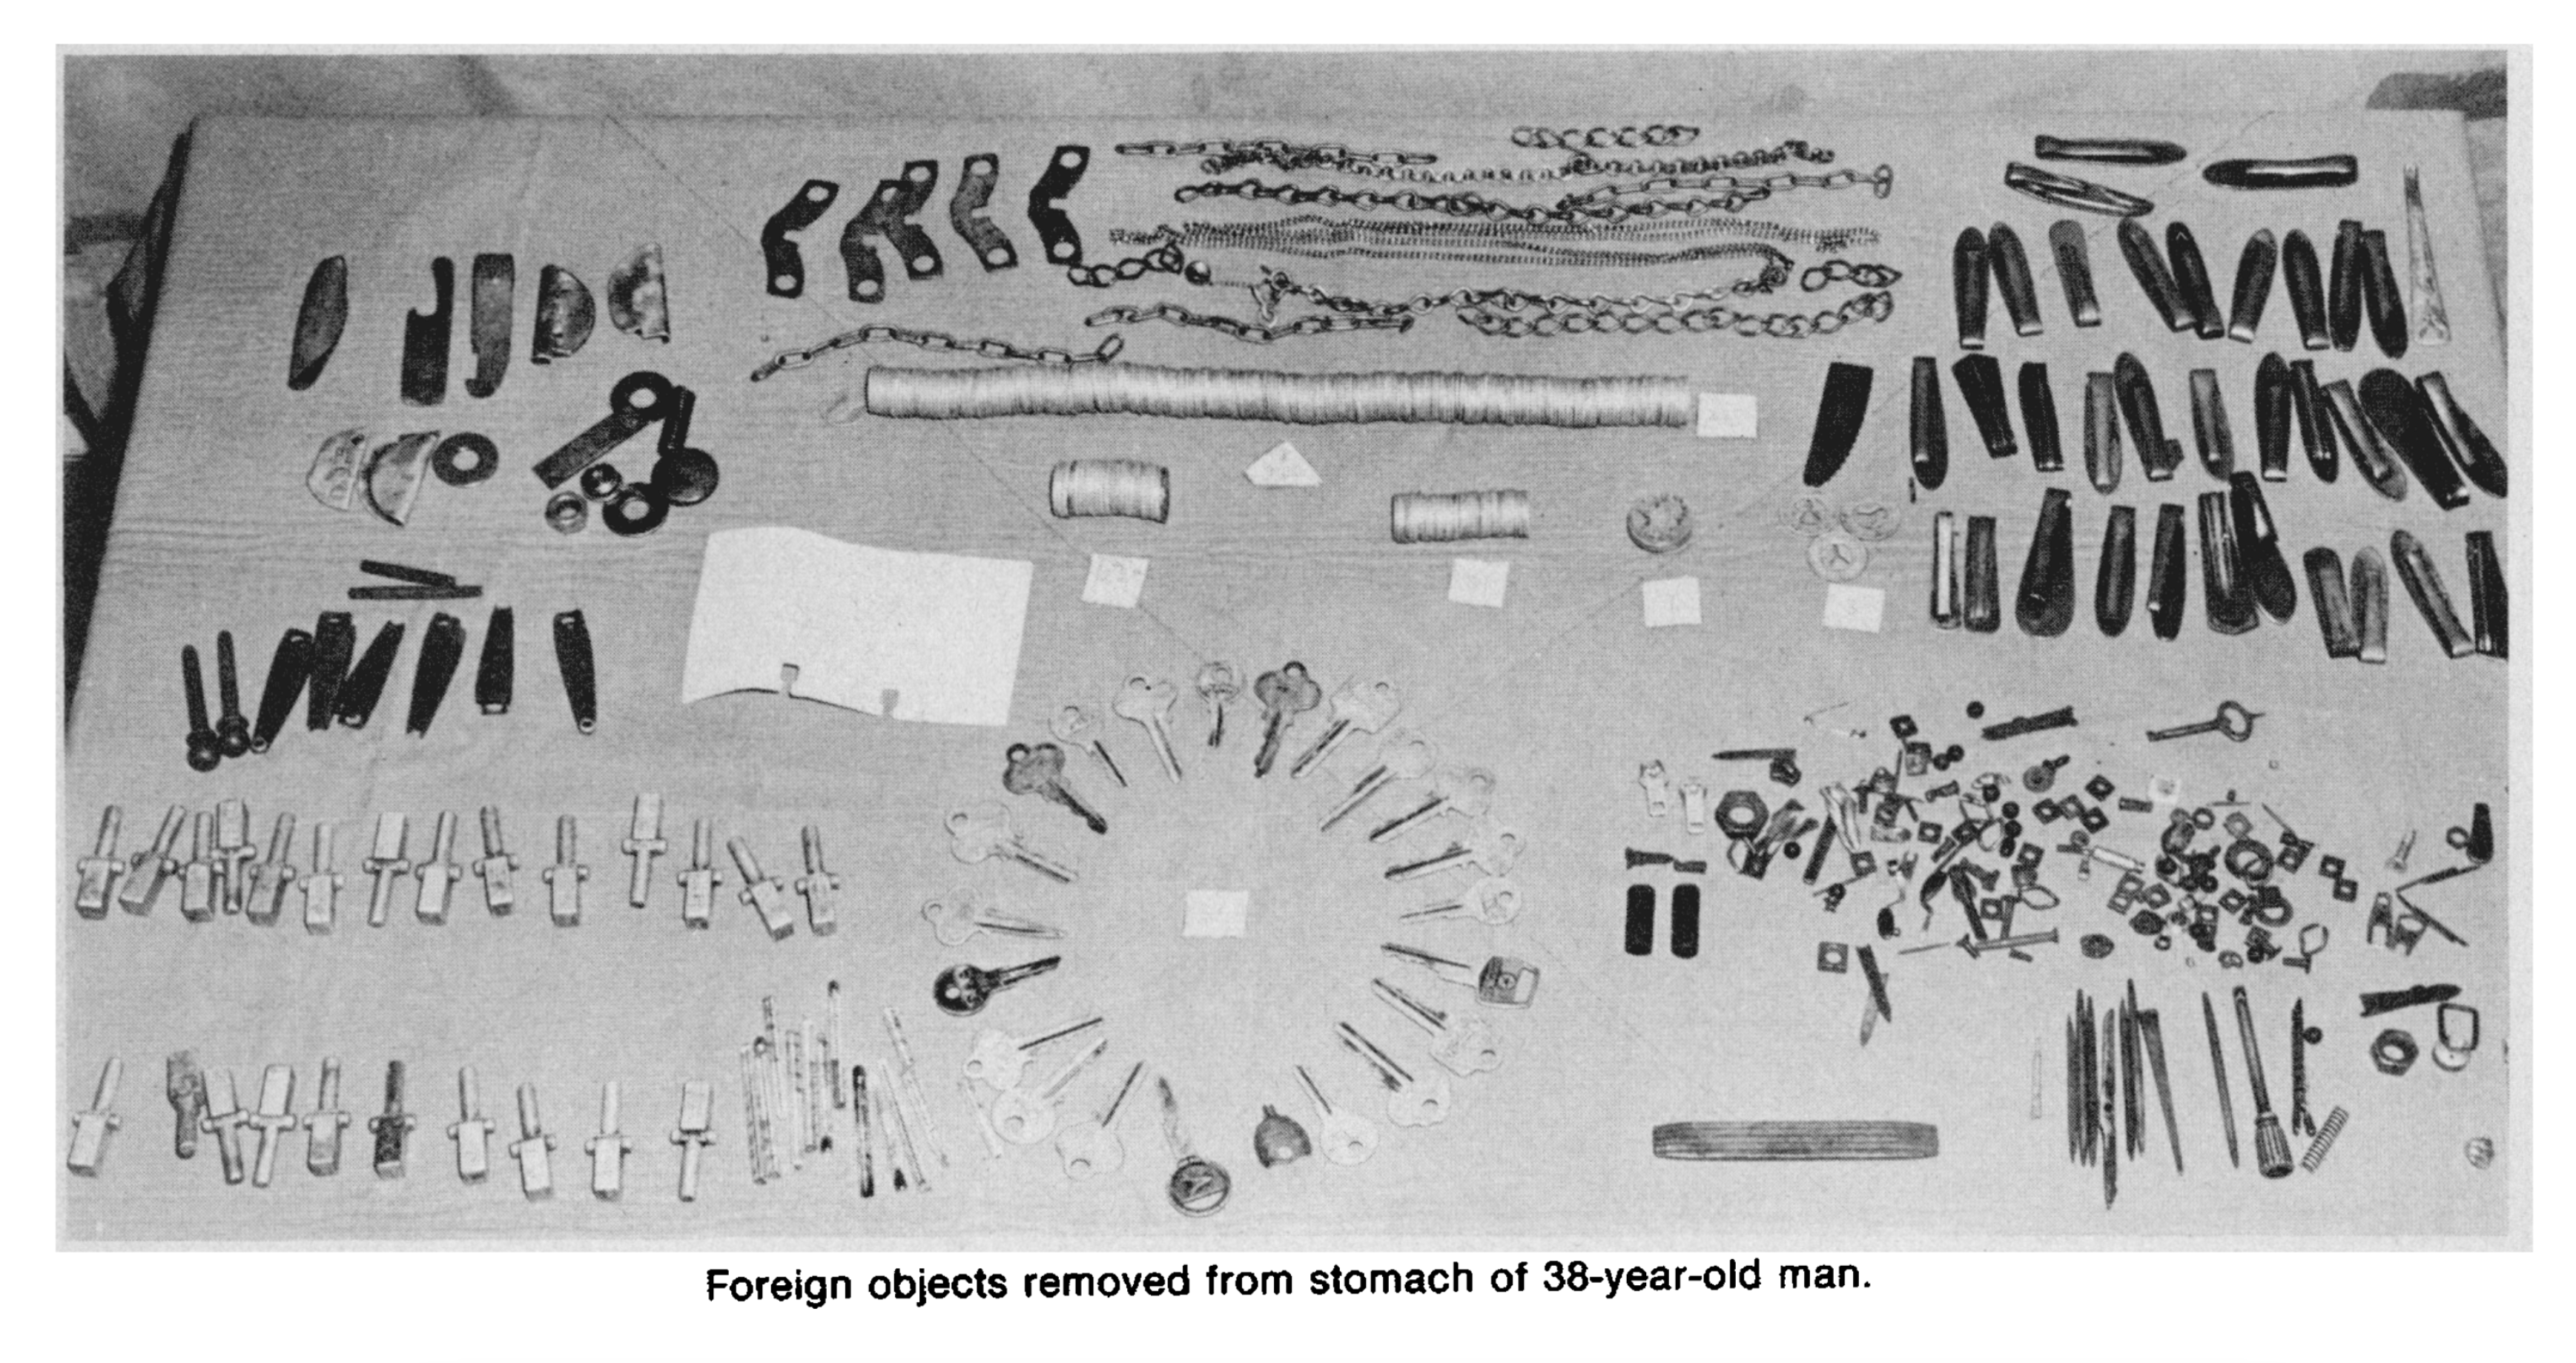
\includegraphics[width=0.8\textwidth]{figures/648_ingested_objects.png}
    \caption{Correlation matrix showing correlation between variables.}
    \label{fig:ingested-metal-obj}
\end{figure}

"We present a case of a patient who ingested 648 metallic objects that formed an intertwining mass within the stomach, requiring operative removal. Of interest was the absence of symptoms and complications after 11 years of continual ingestion. To our knowledge, this is the second heaviest accumulation of metallic foreign objects removed from the stomach of a living patient." \cite{Devanesan_1977}

FOREIGN BODIES IN THE STOMACH: REPORT OF A CASE IN WHICH MORE THAN TWO THOUSAND FIVE HUNDRED FOREIGN BODIES WERE FOUND \cite{Chalk_1928}